% Options for packages loaded elsewhere
\PassOptionsToPackage{unicode}{hyperref}
\PassOptionsToPackage{hyphens}{url}
%
\documentclass[
  11pt,
]{article}
\usepackage{lmodern}
\usepackage{amssymb,amsmath}
\usepackage{ifxetex,ifluatex}
\ifnum 0\ifxetex 1\fi\ifluatex 1\fi=0 % if pdftex
  \usepackage[T1]{fontenc}
  \usepackage[utf8]{inputenc}
  \usepackage{textcomp} % provide euro and other symbols
\else % if luatex or xetex
  \usepackage{unicode-math}
  \defaultfontfeatures{Scale=MatchLowercase}
  \defaultfontfeatures[\rmfamily]{Ligatures=TeX,Scale=1}
\fi
% Use upquote if available, for straight quotes in verbatim environments
\IfFileExists{upquote.sty}{\usepackage{upquote}}{}
\IfFileExists{microtype.sty}{% use microtype if available
  \usepackage[]{microtype}
  \UseMicrotypeSet[protrusion]{basicmath} % disable protrusion for tt fonts
}{}
\makeatletter
\@ifundefined{KOMAClassName}{% if non-KOMA class
  \IfFileExists{parskip.sty}{%
    \usepackage{parskip}
  }{% else
    \setlength{\parindent}{0pt}
    \setlength{\parskip}{6pt plus 2pt minus 1pt}}
}{% if KOMA class
  \KOMAoptions{parskip=half}}
\makeatother
\usepackage{xcolor}
\IfFileExists{xurl.sty}{\usepackage{xurl}}{} % add URL line breaks if available
\IfFileExists{bookmark.sty}{\usepackage{bookmark}}{\usepackage{hyperref}}
\hypersetup{
  hidelinks,
  pdfcreator={LaTeX via pandoc}}
\urlstyle{same} % disable monospaced font for URLs
\usepackage[margin=1.0in]{geometry}
\usepackage{graphicx,grffile}
\makeatletter
\def\maxwidth{\ifdim\Gin@nat@width>\linewidth\linewidth\else\Gin@nat@width\fi}
\def\maxheight{\ifdim\Gin@nat@height>\textheight\textheight\else\Gin@nat@height\fi}
\makeatother
% Scale images if necessary, so that they will not overflow the page
% margins by default, and it is still possible to overwrite the defaults
% using explicit options in \includegraphics[width, height, ...]{}
\setkeys{Gin}{width=\maxwidth,height=\maxheight,keepaspectratio}
% Set default figure placement to htbp
\makeatletter
\def\fps@figure{htbp}
\makeatother
\setlength{\emergencystretch}{3em} % prevent overfull lines
\providecommand{\tightlist}{%
  \setlength{\itemsep}{0pt}\setlength{\parskip}{0pt}}
\setcounter{secnumdepth}{-\maxdimen} % remove section numbering
\usepackage{helvet} % Helvetica font
\renewcommand*\familydefault{\sfdefault} % Use the sans serif version of the font
\usepackage[T1]{fontenc}

\usepackage[none]{hyphenat}

\usepackage{setspace}
\doublespacing
\setlength{\parskip}{1em}

\usepackage{lineno}

\usepackage{pdfpages}

\author{}
\date{\vspace{-2.5em}}

\begin{document}

\vspace{35mm}

\hypertarget{an-osmotic-laxative-renders-mice-susceptible-to-prolonged-clostridioides-difficile-colonization-and-hinders-clearance}{%
\section{\texorpdfstring{An osmotic laxative renders mice susceptible to
prolonged \emph{Clostridioides difficile} colonization and hinders
clearance}{An osmotic laxative renders mice susceptible to prolonged Clostridioides difficile colonization and hinders clearance}}\label{an-osmotic-laxative-renders-mice-susceptible-to-prolonged-clostridioides-difficile-colonization-and-hinders-clearance}}

\vspace{35mm}

Sarah Tomkovich\textsuperscript{1}, Ana Taylor\textsuperscript{1}, Jacob
King\textsuperscript{1}, Joanna Colovas\textsuperscript{1}, Lucas
Bishop\textsuperscript{1}, Kathryn McBride\textsuperscript{1}, Sonya
Royzenblat\textsuperscript{1}, Nicholas A. Lesniak\textsuperscript{1},
Ingrid L. Bergin\textsuperscript{2}, Patrick D.
Schloss\textsuperscript{1\(\dagger\)}

\vspace{40mm}

\(\dagger\) To whom correspondence should be addressed:
\href{mailto:pschloss@umich.edu}{\nolinkurl{pschloss@umich.edu}}

1. Department of Microbiology and Immunology, University of Michigan,
Ann Arbor, MI, USA

2. The Unit for Laboratory Animal Medicine, University of Michigan, Ann
Arbor, MI, USA

\newpage
\linenumbers

\hypertarget{abstract}{%
\subsection{Abstract}\label{abstract}}

(Modify depending on target journal, currently abstract submitted to
World Microbe Forum) Antibiotics are a major risk factor for
\emph{Clostridioides difficile} infections (CDIs) because of their
impact on the intestinal microbiome. However, non-antibiotic medications
such as the ubiquitous osmotic laxative polyethylene glycol (PEG) 3350,
also alter the microbiota, but whether PEG impacts CDI susceptibility
and clearance is unclear. To examine how PEG impacts susceptibility, we
treated C57Bl/6 mice with 5-day and 1-day doses of 15\% PEG in the
drinking water and then challenged the mice with \emph{C. difficile} 630
spores. We used clindamycin-treated mice as a control because they
consistently clear \emph{C. difficile} within 10 days post-infection
(dpi). To examine how PEG treatment impacts clearance, we administered
PEG for 1 day to clindamycin-treated, \emph{C. difficile}-challenged
mice either immediately following challenge or 3 dpi. We collected
longitudinal stool samples to examine \emph{C. difficile} levels in the
stool via anaerobic culture and profiled the microbiota by 16S rRNA
sequencing. PEG treatment alone was sufficient to render mice
susceptible to CDI and 5-day PEG-treated mice remain colonized for up to
30 dpi. Additionally, 5-day PEG treated mice remained susceptible to CDI
10-days post treatment. In contrast, 1-day PEG treated mice were
transiently colonized, clearing \emph{C. difficile} within 7 dpi.
Although 5-day PEG-treated mice exhibited prolonged \emph{C. difficile}
colonization, we saw no difference in histological inflammation between
PEG- and clindamycin-treated mice. Additionally, administering PEG to
mice after \emph{C. difficile} challenge prolonged colonization up to 30
dpi in mice that received PEG immediately after challenge and 15 dpi in
mice that received PEG 3 dpi. When we examined microbiota composition
across our different treatment groups, we found decreased richness in
the PEG-treated mice that exhibited prolonged \emph{C. difficile}
colonization. Importantly, there were increased Bacteroides and
Enterobacteriaceae and decreased Lachnospiraceae and Oscillibacter in
most of the PEG-treated mice with prolonged \emph{C. difficile}
colonization. Our findings suggest the osmotic laxative PEG 3350 alters
the mouse microbiota and disrupts colonization resistance to \emph{C.
difficile}, as well as clearance in mice with a CDI. Considering that
most hospitals recommend not performing \emph{C. difficile} testing on
patients taking laxatives and laxatives are used when administering
fecal microbiota transplants via colonoscopy to patients with recurrent
CDIs, further studies are needed to evaluate if laxatives impact human
microbiota colonization resistance.

\newpage

\hypertarget{introduction}{%
\subsection{Introduction}\label{introduction}}

Antibiotics are a major risk factor for \emph{Clostridioides difficile}
infections (CDIs) because of their impact on the microbiota (1).
However, antibiotics are not the only types of medications that disrupt
the microbiota (2--4). Although, other medications have been implicated
as risk factors for CDIs through epidemiological studies, whether the
association is due to their impact on the microbiome is still unclear
(5--9). Many of the non-antibiotic medications associated with CDIs are
known to modulate intestinal motility, which in turn also strongly
impacts microbiota composition and function (10, 11).

Stool consistency often serves as an approximation of intestinal
motility. Our group has shown that when \emph{C. difficile} negative
controls are separated into two groups based on stool consistency, there
are microbiota features such as alpha diversity that overlap between
samples from CDI patients and control patients with diarrhea (12). These
results led to our hypothesis that bacterial communities from patients
experiencing diarrhea are susceptible, but may not have been exposed to
\emph{C. difficile} spores.

Osmotic laxatives can lead to diarrhea depending on the administered
dose and temporarily disrupts the intestinal microbiota in humans (13).
The ubiquitous osmotic laxative, polyethylene glycol (PEG) 3350 is found
in Miralax, Nulytely, and Golytely and is also commonly used as bowel
preparation for colonoscopies. Interestingly, previous studies have
shown that treating mice with PEG alone rendered the mice susceptible to
\emph{C. difficile} infection, altered microbiota composition, reduced
acetate and butyrate and altered the mucus barrier (14--17). The mucus
barrier is thought to mediate protection from \emph{C. difficile}
infections by protecting intestinal epithelial cells from the toxins
produced by \emph{C. difficile} (Ref). However, whether laxative results
in more severe CDIs in mice is unclear.

Beyond susceptibility, PEG is also relevant in the context of treating
recurrent CDIs via fecal microbiota transplant (FMT) where a healthy
microbiota is administered to the patient to restore colonization. For
FMTs that are delivered via colonoscopy, patients typically undergo
bowel preparation by taking an osmotic laxative prior to the procedure.
Many of the FMT studies to date rationalize the use of laxatives (Ref)
based on a 1996 case study with 2 pediatric patients where the authors
suggested the laxative may help flush \emph{C. difficile} spores and
toxins from the intestine (18).

In the past, our group has used C57BL6 mice to characterize how
antibiotics disrupt the microbiota and influence \emph{C. difficile}
susceptibility and clearance {[}ref{]}. Although, two groups have now
shown PEG treatment alone renders mice susceptible to \emph{C.
difficile}, these studies have raised additional questions that should
be addressed given their relevance to CDIs. Here, we used our C57BL/6
clindamycin model as a control group to characterize how long
PEG-treated mice remain susceptible, whether PEG treatment results in
sustained \emph{C. difficile} colonization, and if PEG treatment
post-CDI can promote \emph{C. difficile} clearance.

\hypertarget{results}{%
\subsection{Results}\label{results}}

\textbf{Laxative treatment alone leads to prolonged \emph{C. difficile}
colonization in mice.} We compared PEG-treated mice to our standard 10
mg/kg clindamycin treatment, which temporarily renders the mice
susceptible to \emph{C. difficile}, with mice typically clearing C.
difficile within 10 days post-infection (9, 19). All PEG-treated mice
were administered a 15\% PEG solution in the drinking water for 5-days,
one group was also treated with clindamycin, and one group was allowed
to recover for 10 days prior to challenge (Fig. 1A). After PEG and/or
antibiotic treatment all mice were challenged with 10\textsuperscript{3}
\emph{C. difficile} 630 spores.

\begin{itemize}
\item
  Figure 1. 5-day PEG treatment prolongs susceptibility and mice become
  persistently colonized with \emph{C. difficile}.
\item
  Figure 2. 5-day PEG treatment disrupts the stool microbiota for a
  longer amount of time compared to clindamycin-treated mice.
\item
  Figure S1. 5-day PEG treatment plus 10-day recovery mice microbiota
  dynamics post-infection.
\item
  Figure 3. 5-day PEG treatment does not result in more severe CDIs,
  although mucosal microbiota is altered.
\item
  Figure 4. 1-day PEG treatment renders mice susceptible to transient
  \emph{C. difficile} colonization.
\item
  Figure 5. 1-day PEG treatment post C. difficile challenge prolongs
  colonization regardless of whether an FMT is also administered.
\item
  Figure 6. Specific microbiota features associated with prolonged
  \emph{C. difficile} colonization in PEG treated mice.
\item
  Figure S2. Specific OTUs associated with clearance that are mostly
  absent in mice with prolonged \emph{C. difficile} colonization.

  \begin{itemize}
  \tightlist
  \item
    Ex. \emph{Muribaculum intestinale}.
  \end{itemize}
\item
  Figure 7. Schematic summarizing findings.
\end{itemize}

\hypertarget{discussion}{%
\subsection{Discussion}\label{discussion}}

\begin{itemize}
\item
  Summary of major findings
\item
  Discussion of prolonged persistence. C. difficile sequences detected
  in tissue samples. Association with mucin-degrading bacteria suggested
  by recent papers.
\item
  Discuss why we might not have observed more severe histology in PEG
  mice relative to clindamycin-treated mice

  \begin{itemize}
  \tightlist
  \item
    Antibiotics may also impact mucus layer
  \item
    Strain of bacteria used
  \end{itemize}
\item
  Protective bacteria missing in PEG-treated mice
\item
  Discuss what these findings might mean for human patients

  \begin{itemize}
  \tightlist
  \item
    What's known regarding laxatives and susceptibility to CDIs
  \item
    Relevance to human FMTs? Unclear what the best administration route
    is because there have been no studies designed to evaluate the best
    administration route for FMTs.
  \end{itemize}
\end{itemize}

\hypertarget{conclusions}{%
\subsection{Conclusions}\label{conclusions}}

\hypertarget{acknowledgements}{%
\subsection{Acknowledgements}\label{acknowledgements}}

We thank members of the Schloss lab for feedback on planning the
experiments and data presentation. We also thank Andrew Henry for help
with media preparation and bacterial culture. We also thank the Unit for
Laboratory Animal Medicine at the University of Michigan for maintaining
our mouse colony and providing the institutional support for our mouse
experiments. Finally, we thank Kwi Kim, Austin Campbell, and Kimberly
Vendrov for their help in maintaining the Schloss lab's anaerobic
chamber. This work was supported by the National Institutes of Health
(U01AI124255). ST was supported by the Michigan Institute for Clincial
and Health Research Postdoctoral Translation Scholars Program
(UL1TR002240 from the National Center for Advancing Translational
Sciences).

\hypertarget{materials-and-methods}{%
\subsection{Materials and Methods}\label{materials-and-methods}}

\newpage

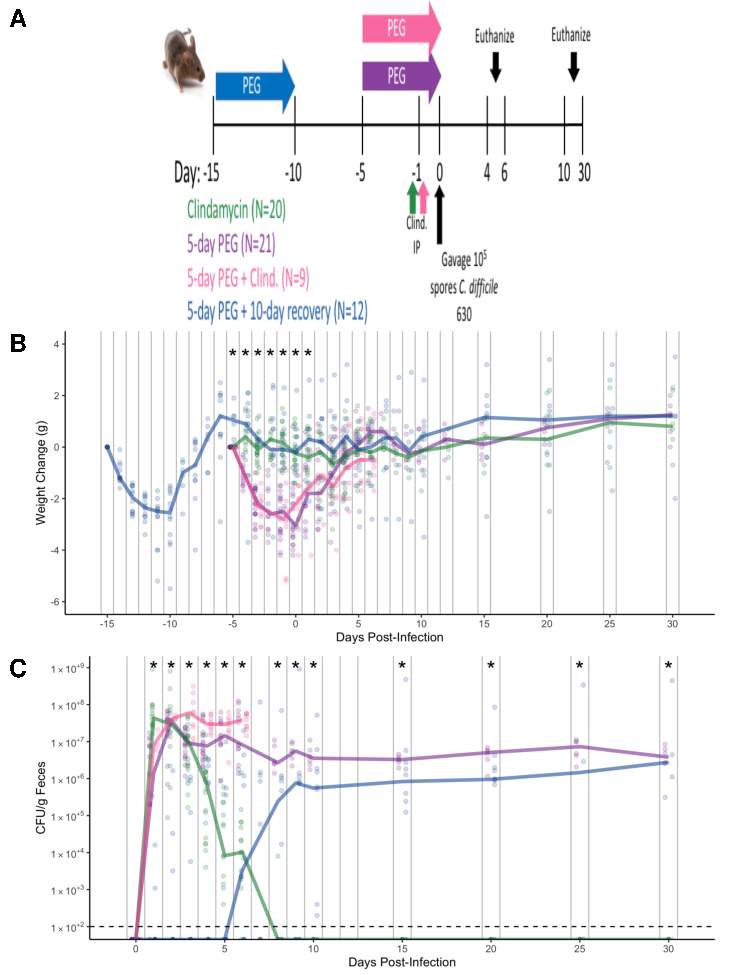
\includegraphics{figure_1.pdf}

\textbf{Figure 1. 5-day PEG treatment prolongs susceptibility and mice
become persistently colonized with \emph{C. difficile}.} A. Setup of the
experimental timeline for subset of experiments with 5-day PEG treated
mice. B. Weight change from baseline weight in groups after treatment
with PEG and/or clindamycin, followed by \emph{C. difficile} challenge.
C. \emph{C. difficile} CFU/gram stool measured over time (N =
4-\texttt{(insert\ variable\ name)} mice per timepoint) via serial
dilutions. The black line represents the limit of detection for the
first serial dilution. CFU quantification data was not available for
each mouse due to stool sampling difficulties (particularly the day the
mice came off of the PEG treatment) or early deaths. Lines represent the
median for each source and circles represent individual mouse samples.
Asterisks indicate timepoints where the weight change or CFU/g was
significantly different between groups by the Kruskal-Wallis test with
Benjamini-Hochberg correction for testing multiple timepoints. \newpage

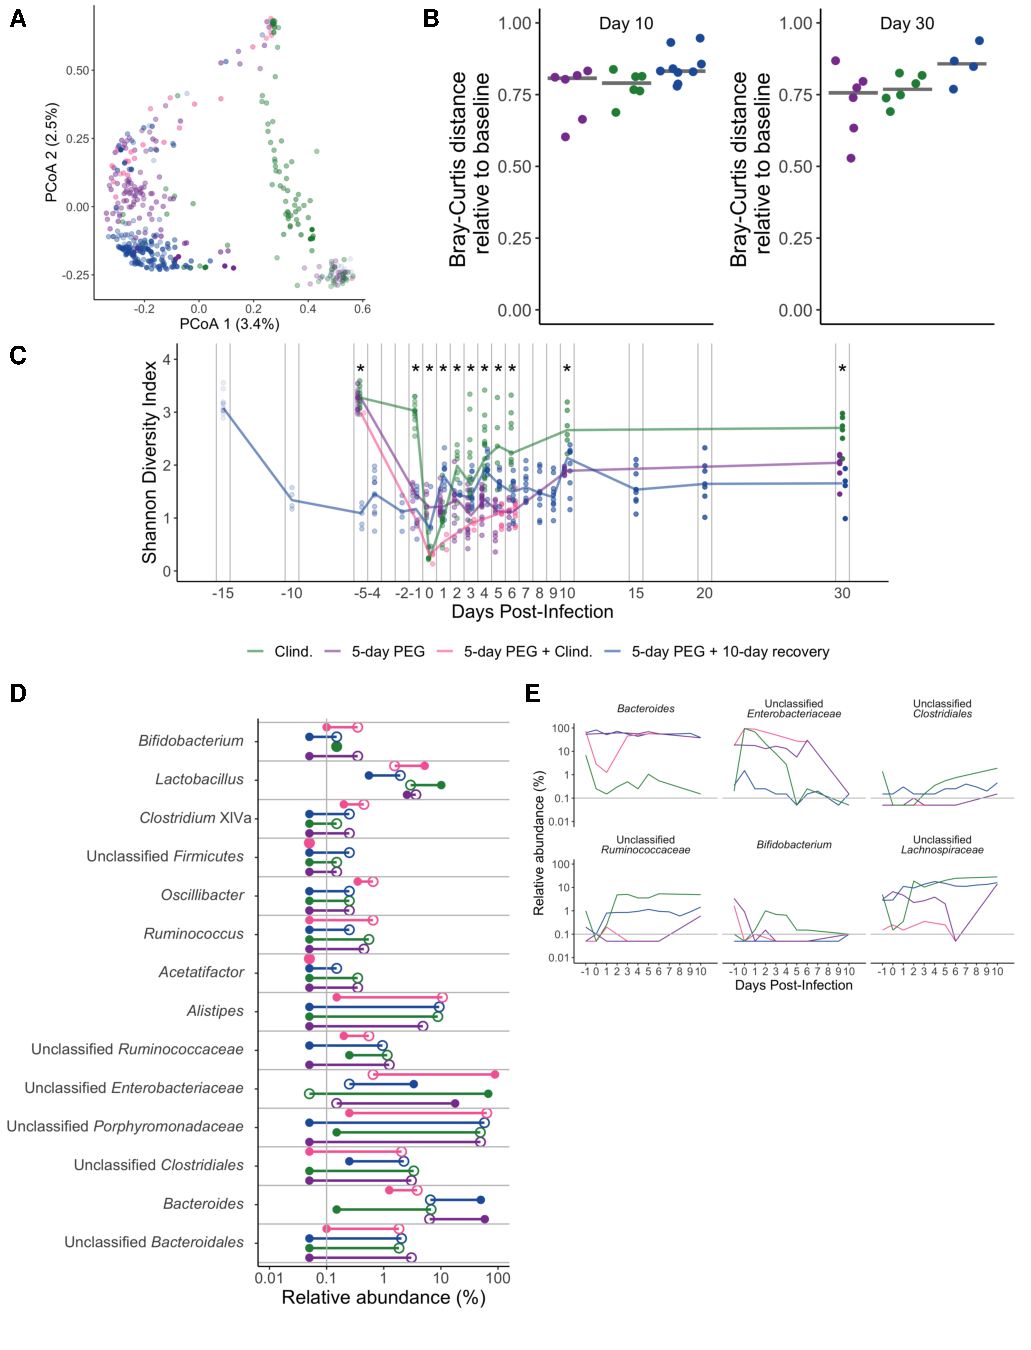
\includegraphics{figure_2.pdf} \textbf{Figure 2. 5-day PEG treatment
disrupts the stool microbiota for a longer amount of time compared to
clindamycin-treated mice.} A. \newpage

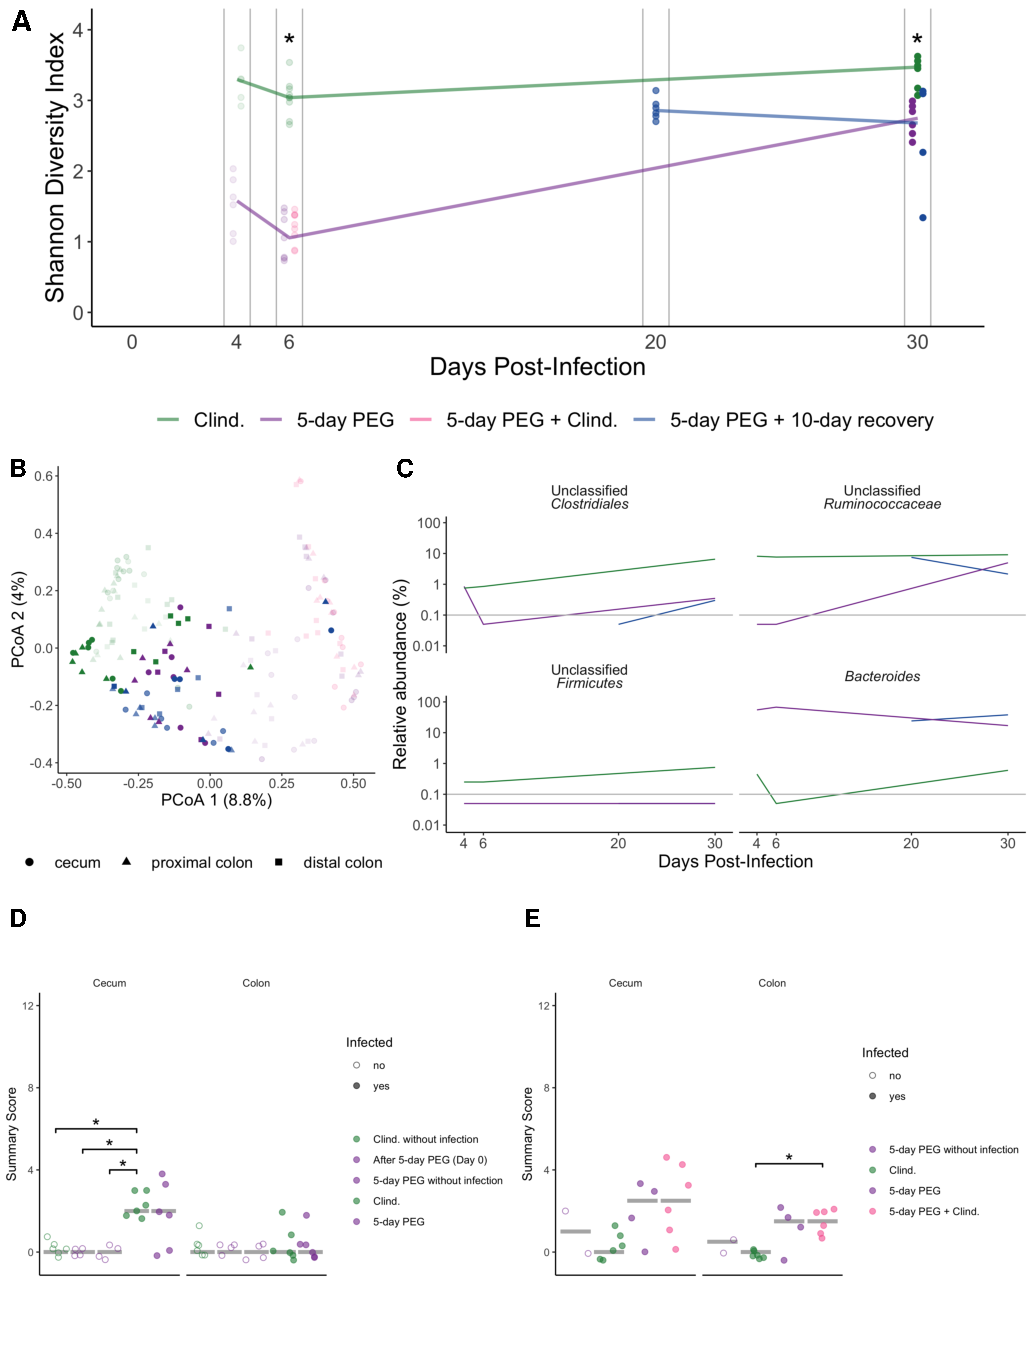
\includegraphics{figure_3.pdf} \textbf{Figure 3. 5-day PEG treatment
does not result in more severe CDIs, although mucosal microbiota is
altered.} A. \newpage

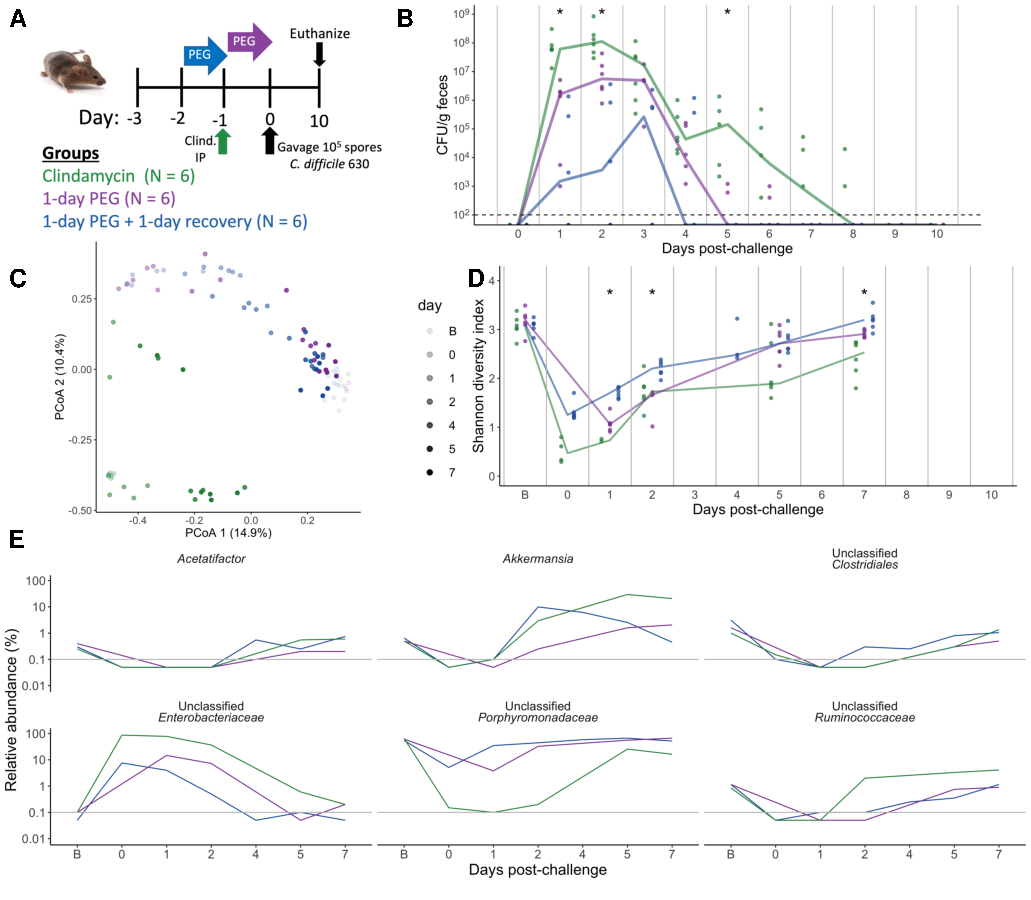
\includegraphics{figure_4.pdf} \textbf{Figure 4. 1-day PEG treatment
renders mice susceptible to transient \emph{C. difficile} colonization.}
A. Setup of the experimental timeline for the 1-day PEG treated subset
of mice. B. CFU/gram stool measured over time (N = 6 mice per timepoint)
via several dilutions. The black dotted line represents the limit of
detection for the first serial dilution. Asterisks indicate timepoints
where the CFU/gram was siginificantly different between groups using the
Kruskall-Wallis test with a Benjamini-Hochberg correction for multiple
timepoints. C. Principle Coordinate Analysis plot of the groups over
time with the alpha representating the same time scale as in panel D
(day: R\textsuperscript{2} = 0.43; group: R\textsuperscript{2} = 0.19).
D. Shannon Diveristy Index of the groups over time. Only days with
samples from all groups are shown. Samples for some mice were difficult
to obtain due to the laxative treatment. The alpha scale follows
accordingly with the timeline. E. Line plots of relative percent
abundance of selected genera over time. Only days with samples from all
groups shown. The gray line represents the limit of detection.

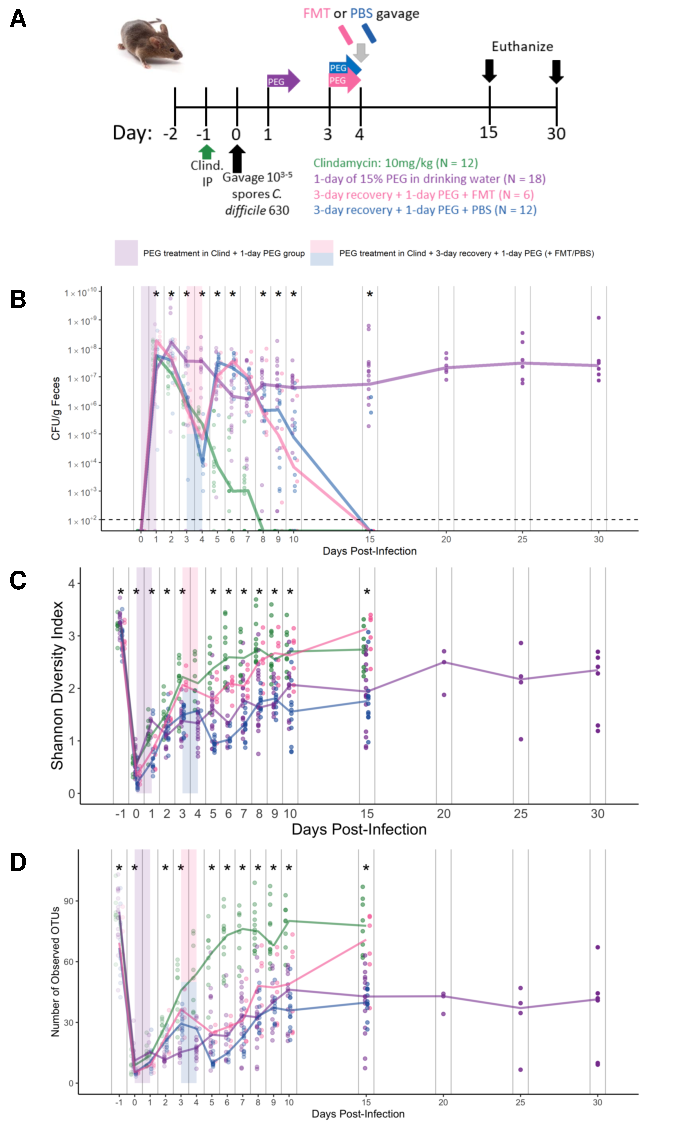
\includegraphics{figure_5.pdf} 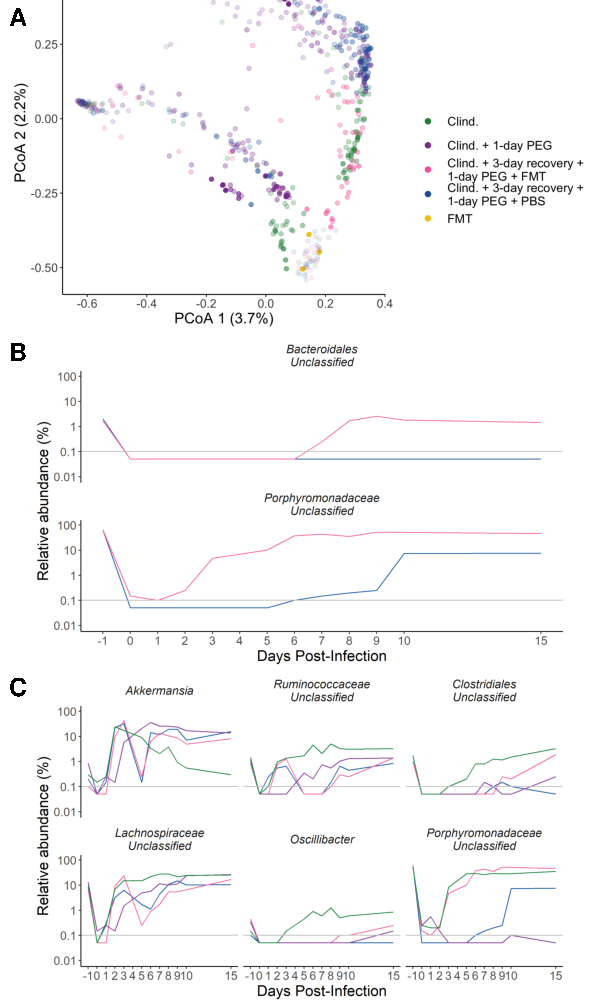
\includegraphics{figure_5_16S.pdf}
\textbf{Figure 5. 1-day PEG treatment post C. difficile challenge
prolongs colonization regardless of whether an FMT is also
administered.} A. \newpage

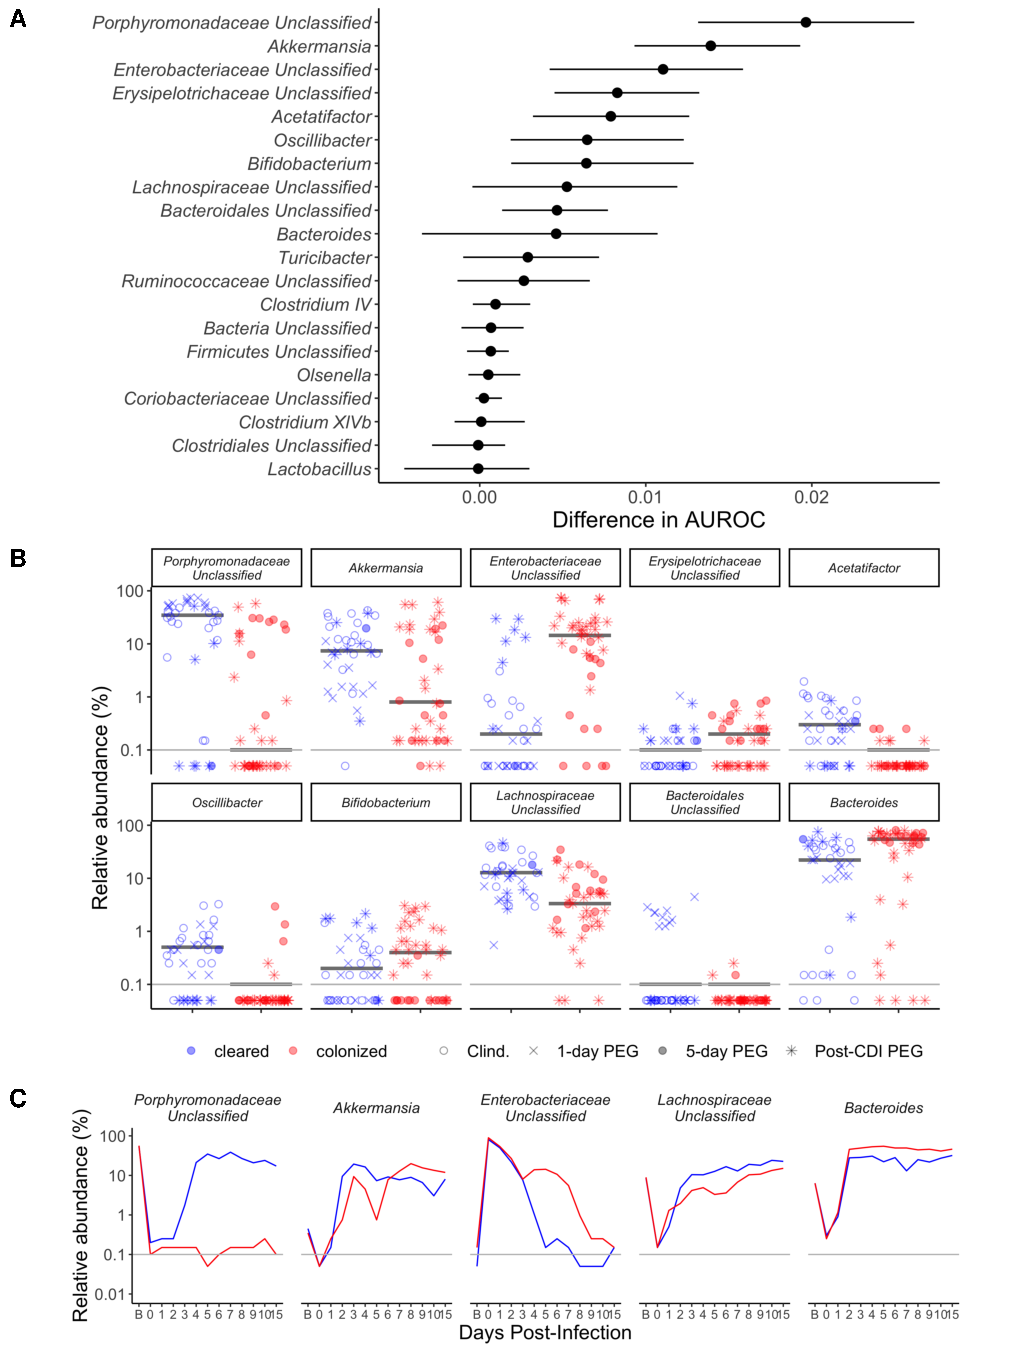
\includegraphics{figure_6.pdf} \textbf{Figure 6. Specific microbiota
features associated with prolonged \emph{C. difficile} colonization in
PEG treated mice.} A. \newpage

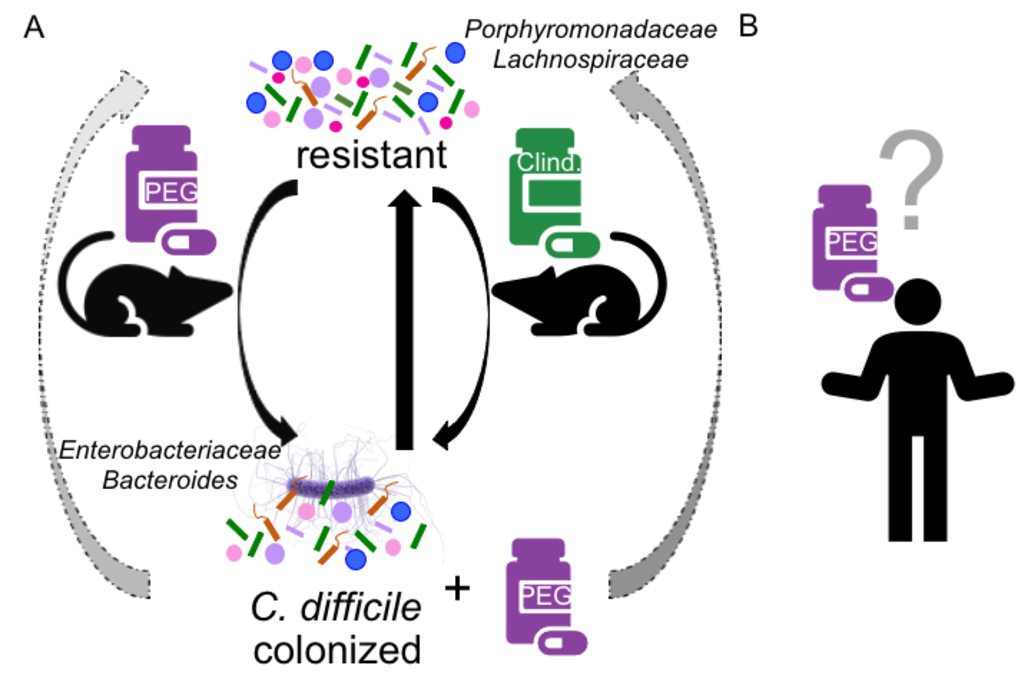
\includegraphics{figure_7.pdf} \textbf{Figure 7. Schematic summarizing
findings.} A. \newpage

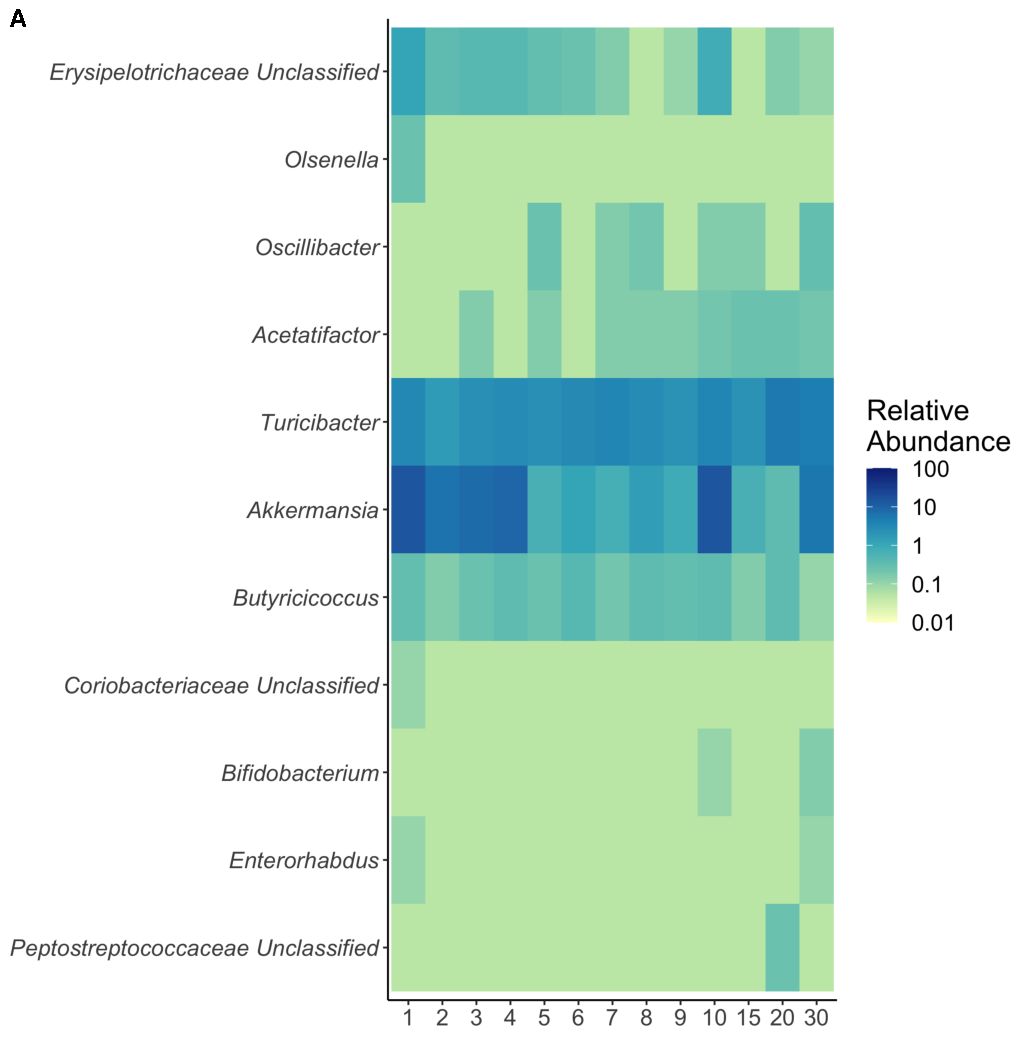
\includegraphics{figure_S1.pdf} \textbf{Figure S1. 5-day PEG treatment
plus 10-day recovery mice microbiota dynamics post-infection.} A.
\newpage

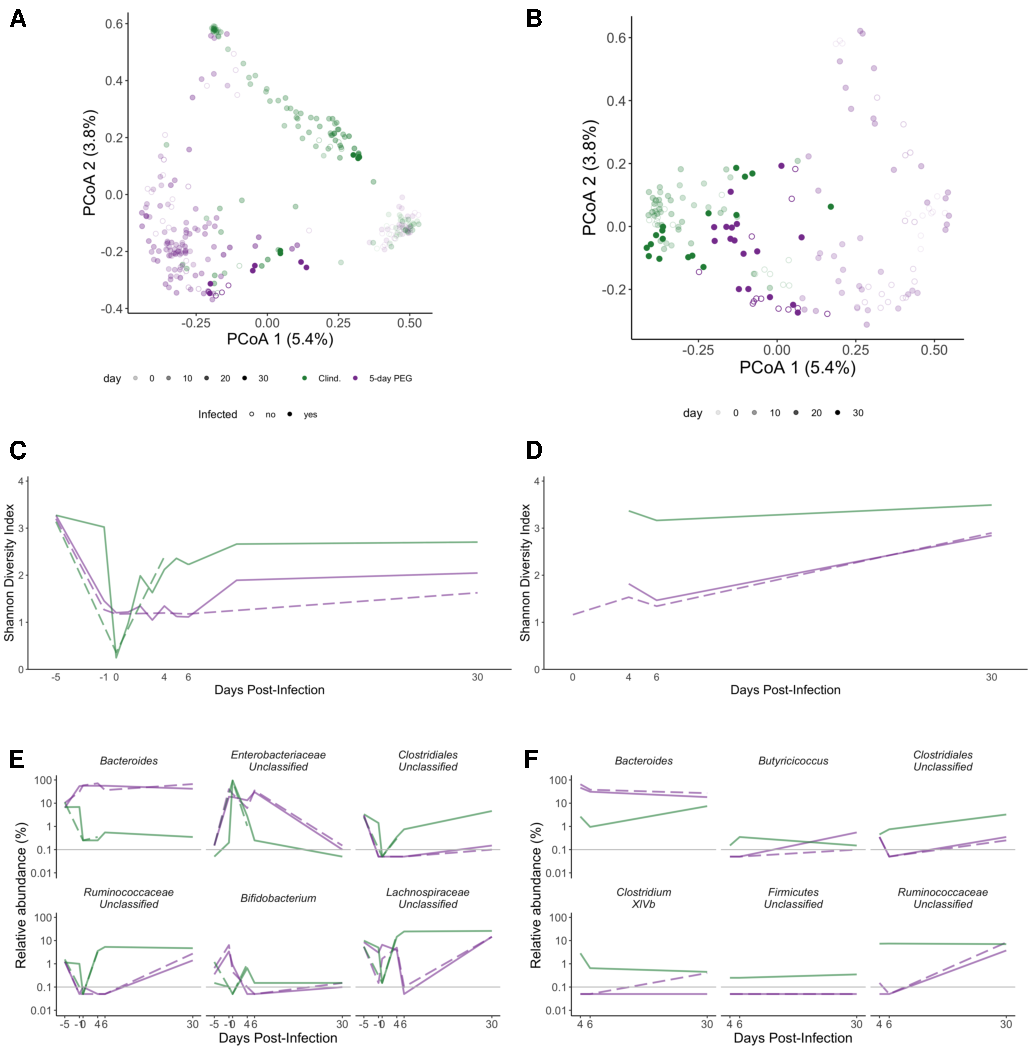
\includegraphics{figure_S2.pdf} \textbf{Figure S2. Specific OTUs
associated with clearance that are mostly absent in mice with prolonged
\emph{C. difficile} colonization. Ex. \emph{Muribaculum intestinale}.}
A. \newpage

\hypertarget{references}{%
\subsection*{References}\label{references}}
\addcontentsline{toc}{subsection}{References}

\hypertarget{refs}{}
\leavevmode\hypertarget{ref-Britton2014}{}%
1. \textbf{Britton RA}, \textbf{Young VB}. 2014. Role of the intestinal
microbiota in resistance to colonization by clostridium difficile.
Gastroenterology \textbf{146}:1547--1553.
doi:\href{https://doi.org/10.1053/j.gastro.2014.01.059}{10.1053/j.gastro.2014.01.059}.

\leavevmode\hypertarget{ref-Maier2018}{}%
2. \textbf{Maier L}, \textbf{Pruteanu M}, \textbf{Kuhn M},
\textbf{Zeller G}, \textbf{Telzerow A}, \textbf{Anderson EE},
\textbf{Brochado AR}, \textbf{Fernandez KC}, \textbf{Dose H},
\textbf{Mori H}, \textbf{Patil KR}, \textbf{Bork P}, \textbf{Typas A}.
2018. Extensive impact of non-antibiotic drugs on human gut bacteria.
Nature \textbf{555}:623--628.
doi:\href{https://doi.org/10.1038/nature25979}{10.1038/nature25979}.

\leavevmode\hypertarget{ref-LeBastard2017}{}%
3. \textbf{Bastard QL}, \textbf{Al-Ghalith GA}, \textbf{Grégoire M},
\textbf{Chapelet G}, \textbf{Javaudin F}, \textbf{Dailly E},
\textbf{Batard E}, \textbf{Knights D}, \textbf{Montassier E}. 2017.
Systematic review: Human gut dysbiosis induced by non-antibiotic
prescription medications. Alimentary Pharmacology \& Therapeutics
\textbf{47}:332--345.
doi:\href{https://doi.org/10.1111/apt.14451}{10.1111/apt.14451}.

\leavevmode\hypertarget{ref-VichVila2020}{}%
4. \textbf{Vila AV}, \textbf{Collij V}, \textbf{Sanna S}, \textbf{Sinha
T}, \textbf{Imhann F}, \textbf{Bourgonje AR}, \textbf{Mujagic Z},
\textbf{Jonkers DMAE}, \textbf{Masclee AAM}, \textbf{Fu J},
\textbf{Kurilshikov A}, \textbf{Wijmenga C}, \textbf{Zhernakova A},
\textbf{Weersma RK}. 2020. Impact of commonly used drugs on the
composition and metabolic function of the gut microbiota. Nature
Communications \textbf{11}.
doi:\href{https://doi.org/10.1038/s41467-019-14177-z}{10.1038/s41467-019-14177-z}.

\leavevmode\hypertarget{ref-Oh2018}{}%
5. \textbf{Oh J}, \textbf{Makar M}, \textbf{Fusco C}, \textbf{McCaffrey
R}, \textbf{Rao K}, \textbf{Ryan EE}, \textbf{Washer L}, \textbf{West
LR}, \textbf{Young VB}, \textbf{Guttag J}, \textbf{Hooper DC},
\textbf{Shenoy ES}, \textbf{Wiens J}. 2018. A generalizable, data-driven
approach to predict daily risk ofClostridium difficileInfection at two
large academic health centers. Infection Control \& Hospital
Epidemiology \textbf{39}:425--433.
doi:\href{https://doi.org/10.1017/ice.2018.16}{10.1017/ice.2018.16}.

\leavevmode\hypertarget{ref-Mora2012}{}%
6. \textbf{Mora AL}, \textbf{Salazar M}, \textbf{Pablo-Caeiro J},
\textbf{Frost CP}, \textbf{Yadav Y}, \textbf{DuPont HL}, \textbf{Garey
KW}. 2012. Moderate to high use of opioid analgesics are associated with
an increased risk of clostridium difficile infection. The American
Journal of the Medical Sciences \textbf{343}:277--280.
doi:\href{https://doi.org/10.1097/maj.0b013e31822f42eb}{10.1097/maj.0b013e31822f42eb}.

\leavevmode\hypertarget{ref-Nehra2018}{}%
7. \textbf{Nehra AK}, \textbf{Alexander JA}, \textbf{Loftus CG},
\textbf{Nehra V}. 2018. Proton pump inhibitors: Review of emerging
concerns. Mayo Clinic Proceedings \textbf{93}:240--246.
doi:\href{https://doi.org/10.1016/j.mayocp.2017.10.022}{10.1016/j.mayocp.2017.10.022}.

\leavevmode\hypertarget{ref-Krishna2013}{}%
8. \textbf{Krishna SG}, \textbf{Zhao W}, \textbf{Apewokin SK},
\textbf{Krishna K}, \textbf{Chepyala P}, \textbf{Anaissie EJ}. 2013.
Risk factors, preemptive therapy, and antiperistaltic agents
forClostridium difficileinfection in cancer patients. Transplant
Infectious Disease n/a--n/a.
doi:\href{https://doi.org/10.1111/tid.12112}{10.1111/tid.12112}.

\leavevmode\hypertarget{ref-Tomkovich2019}{}%
9. \textbf{Tomkovich S}, \textbf{Lesniak NA}, \textbf{Li Y},
\textbf{Bishop L}, \textbf{Fitzgerald MJ}, \textbf{Schloss PD}. 2019.
The proton pump inhibitor omeprazole does not promote
\emph{Clostridioides difficile} colonization in a murine model. mSphere
\textbf{4}.
doi:\href{https://doi.org/10.1128/msphere.00693-19}{10.1128/msphere.00693-19}.

\leavevmode\hypertarget{ref-Vandeputte2015}{}%
10. \textbf{Vandeputte D}, \textbf{Falony G}, \textbf{Vieira-Silva S},
\textbf{Tito RY}, \textbf{Joossens M}, \textbf{Raes J}. 2015. Stool
consistency is strongly associated with gut microbiota richness and
composition, enterotypes and bacterial growth rates. Gut
\textbf{65}:57--62.
doi:\href{https://doi.org/10.1136/gutjnl-2015-309618}{10.1136/gutjnl-2015-309618}.

\leavevmode\hypertarget{ref-VujkovicCvijin2020}{}%
11. \textbf{Vujkovic-Cvijin I}, \textbf{Sklar J}, \textbf{Jiang L},
\textbf{Natarajan L}, \textbf{Knight R}, \textbf{Belkaid Y}. 2020. Host
variables confound gut microbiota studies of human disease. Nature
\textbf{587}:448--454.
doi:\href{https://doi.org/10.1038/s41586-020-2881-9}{10.1038/s41586-020-2881-9}.

\leavevmode\hypertarget{ref-Schubert2015}{}%
12. \textbf{Schubert AM}, \textbf{Sinani H}, \textbf{Schloss PD}. 2015.
Antibiotic-induced alterations of the murine gut microbiota and
subsequent effects on colonization resistance against \emph{Clostridium
difficile}. mBio \textbf{6}.
doi:\href{https://doi.org/10.1128/mbio.00974-15}{10.1128/mbio.00974-15}.

\leavevmode\hypertarget{ref-Nagata2019}{}%
13. \textbf{Nagata N}, \textbf{Tohya M}, \textbf{Fukuda S}, \textbf{Suda
W}, \textbf{Nishijima S}, \textbf{Takeuchi F}, \textbf{Ohsugi M},
\textbf{Tsujimoto T}, \textbf{Nakamura T}, \textbf{Shimomura A},
\textbf{Yanagisawa N}, \textbf{Hisada Y}, \textbf{Watanabe K},
\textbf{Imbe K}, \textbf{Akiyama J}, \textbf{Mizokami M},
\textbf{Miyoshi-Akiyama T}, \textbf{Uemura N}, \textbf{Hattori M}. 2019.
Effects of bowel preparation on the human gut microbiome and metabolome.
Scientific Reports \textbf{9}.
doi:\href{https://doi.org/10.1038/s41598-019-40182-9}{10.1038/s41598-019-40182-9}.

\leavevmode\hypertarget{ref-Kashyap2013}{}%
14. \textbf{Kashyap PC}, \textbf{Marcobal A}, \textbf{Ursell LK},
\textbf{Larauche M}, \textbf{Duboc H}, \textbf{Earle KA},
\textbf{Sonnenburg ED}, \textbf{Ferreyra JA}, \textbf{Higginbottom SK},
\textbf{Million M}, \textbf{Tache Y}, \textbf{Pasricha PJ},
\textbf{Knight R}, \textbf{Farrugia G}, \textbf{Sonnenburg JL}. 2013.
Complex interactions among diet, gastrointestinal transit, and gut
microbiota in humanized mice. Gastroenterology \textbf{144}:967--977.
doi:\href{https://doi.org/10.1053/j.gastro.2013.01.047}{10.1053/j.gastro.2013.01.047}.

\leavevmode\hypertarget{ref-Ferreyra2014}{}%
15. \textbf{Ferreyra JA}, \textbf{Wu KJ}, \textbf{Hryckowian AJ},
\textbf{Bouley DM}, \textbf{Weimer BC}, \textbf{Sonnenburg JL}. 2014.
Gut microbiota-produced succinate promotes c.~difficile infection after
antibiotic treatment or motility disturbance. Cell Host \& Microbe
\textbf{16}:770--777.
doi:\href{https://doi.org/10.1016/j.chom.2014.11.003}{10.1016/j.chom.2014.11.003}.

\leavevmode\hypertarget{ref-Tropini2018}{}%
16. \textbf{Tropini C}, \textbf{Moss EL}, \textbf{Merrill BD},
\textbf{Ng KM}, \textbf{Higginbottom SK}, \textbf{Casavant EP},
\textbf{Gonzalez CG}, \textbf{Fremin B}, \textbf{Bouley DM},
\textbf{Elias JE}, \textbf{Bhatt AS}, \textbf{Huang KC},
\textbf{Sonnenburg JL}. 2018. Transient osmotic perturbation causes
long-term alteration to the gut microbiota. Cell
\textbf{173}:1742--1754.e17.
doi:\href{https://doi.org/10.1016/j.cell.2018.05.008}{10.1016/j.cell.2018.05.008}.

\leavevmode\hypertarget{ref-VanInsberghe2020}{}%
17. \textbf{VanInsberghe D}, \textbf{Elsherbini JA}, \textbf{Varian B},
\textbf{Poutahidis T}, \textbf{Erdman S}, \textbf{Polz MF}. 2020.
Diarrhoeal events can trigger long-term clostridium difficile
colonization with recurrent blooms. Nature Microbiology
\textbf{5}:642--650.
doi:\href{https://doi.org/10.1038/s41564-020-0668-2}{10.1038/s41564-020-0668-2}.

\leavevmode\hypertarget{ref-Liacouras1996}{}%
18. \textbf{Liacouras CA}, \textbf{Piccoli DA}. 1996. Whole-bowel
irrigation as an adjunct to the treatment of chronic, relapsing
clostridium difficile colitis. Journal of Clinical Gastroenterology
\textbf{22}:186--189.
doi:\href{https://doi.org/10.1097/00004836-199604000-00007}{10.1097/00004836-199604000-00007}.

\leavevmode\hypertarget{ref-Tomkovich2020}{}%
19. \textbf{Tomkovich S}, \textbf{Stough JMA}, \textbf{Bishop L},
\textbf{Schloss PD}. 2020. The initial gut microbiota and response to
antibiotic perturbation influence clostridioides difficile clearance in
mice. mSphere \textbf{5}.
doi:\href{https://doi.org/10.1128/msphere.00869-20}{10.1128/msphere.00869-20}.

\end{document}
